\documentclass{article}
\usepackage{graphicx}% Required for inserting images
\usepackage{lindrew}
\usepackage[shortlabels]{enumitem}
\usepackage{enumerate}
\usepackage{algorithm}
\usepackage{algpseudocode}
\usepackage{matlab-prettifier}
\usepackage{pythonhighlight}

\title{CS 156a Problem Set 4}
\author{Amitesh Anand Pandey}
\date{October 2024}

\begin{document}
\maketitle
\section*{Generalization Error}
\subsection*{Problem 1}
We know that the generalization bound is
\begin{equation*}
\epsilon = \sqrt{\frac{8}{N}\ln \left(\frac{4m_{\mathcal{H}}(2N)}{\delta}\right)}
\end{equation*}
where $\epsilon$ is our tolerance towards the discrepancy in $E_{in}$ and $E_{out}$ and $1-\delta$ is our confidence in meeting this tolerance. Then we can substitute $m_{\mathcal{H}}(2N) = (2N)^{d_{\text{VC}}} = (2N)^{10} = 2^{10}N^{10}$, $\epsilon = 0.05$, $\delta = 1-0.95 = 0.05$, we get
\begin{equation*}
0.05 = \sqrt{\frac{8}{N}\ln \left(\frac{4\cdot 2^{10}N^{10}}{0.05}\right)}
\end{equation*}
Then
\begin{equation*}
    0.0025N = 8\ln\left(\frac{4 \cdot 2^{10}N^{10}}{0.05}\right)
\end{equation*}
\begin{equation*}
    \frac{0.0025}{8}N = \ln{\left(\frac{4\cdot 2^{10}N^{10}}{0.05}\right)}
\end{equation*}
Raising both sides with base power $e$,
\begin{equation*}
    (1.00031254883)^{N} = \frac{4\cdot 2^{10}N^{10}}{0.05}
\end{equation*}
Using the \hyperref[prob1]{code} We get $N \approx 452957$, thus $N = 460000$, option $[\textbf{d}]$ is correct.\newpage
\subsection*{Problem 2}
So for a hypothesis set $\mathcal{H}$ with $d_{\text{VC}} = 50$, setting $\delta = 0.05$, we get the following plots:
\begin{figure}[htp]
    \centering
    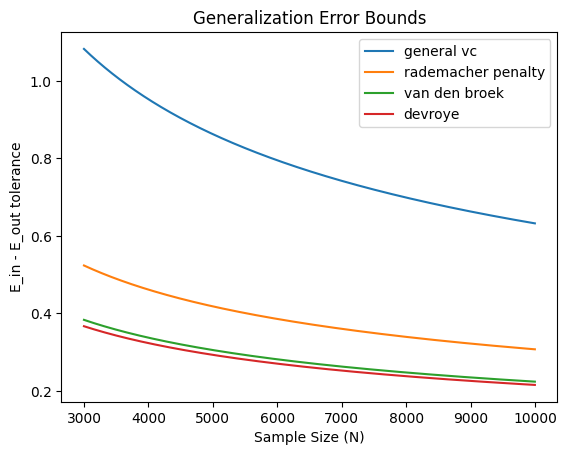
\includegraphics[width=3in]{plotps4.png}
    \label{fig:galaxy}
\end{figure}
\noindent{From } this, it is clear that at $N=10000$, Devroye bound is the smallest so $\textbf{[d]}$ is the correct option, using this \hyperref[prob2]{code} implemented in Python.
\subsection*{Problem 3}
For $n = 5$, the Van den Broek bound is the smallest, so $\textbf{[c]}$ is the correct option.
\section*{Bias and Variance}
\subsection*{Problem 4}
For this problem, for two points $(x_{1}, \sin(\pi x_{1})), (x_{2}, \sin{(\pi x_{2}}))$, I calculated the mean square error of all hypotheses $g(x) = ax$ for $a = 0.000,0.001,\dots 9.999$. Then I picked the $a$ (slope) that minimized the mean square error. I repeated this experiment 10000 times and took the mean slope. I got $\hat{a} \approx 1.42$, so $\textbf{[e]}$ is the correct option. Using this \hyperref[prob4]{code} in Python.
\subsection*{Problem 5}
For the bias $b$, we have
\begin{equation*}
    b = \mathbb{E}_{x}\left[(\Bar{g}(x) - f(x))^{2}\right]
\end{equation*}
where $\Bar{g}(x) = 1.42x$ and $f(x) = \sin{(\pi x)}$. Remember that in a real-world problem, an expression for $f(x)$ is not \emph{a priori} available, however this value can still be determined using enough $(x,y)$ pairs out of sample. In our case, we can simply substitute the analytic expression for $f(x)$ since generating these pairs through this function would serve the same purpose. Then
\begin{equation*}
    b = \frac{1}{2}\int_{-1}^{1}(1.42x - \sin{(\pi x)})^2\text{d}x = \frac{1}{2}\cdot 0.536 \approx 0.265
\end{equation*}
So $\textbf{[b]}$ is the correct option.
\newpage
\subsection*{Problem 6}
For the variance $v$, we have
\begin{equation*}
    v = \mathbb{E}_{x}\left[\mathbb{E}_{\mathcal{D}}\left[(g^{\mathcal{(D)}}(x) - \Bar{g}(x))^{2}\right]\right]
\end{equation*}
We already know $\Bar{g}(x) = 1.42x$, but $g^{(\mathcal{D})}$ obviously depends on the dataset $\mathcal{D}$. So let's get the best hypotheses $g^{(\mathcal{D}_1)}, g^{(\mathcal{D}_2)}, \dots, g^{(\mathcal{D}_{1000})}$, for 1000 datasets, and then compute the mean value of the variance. On doing so, we get
\begin{equation*}
    v = \mathbb{E}_{x}\left[(0.71x)^{2}\right] = \frac{1}{2}\int_{-1}^{1}0.53x^2\text{d}x = \frac{1}{2}\cdot 0.36 = 0.18
\end{equation*}
Thus the correct option is $[\textbf{a}]$. Essentially, we are using two points $(x_{1}, y_{1}), (x_{2}, y_{2}) \in \mathcal{D}_{n}$ to generate a best hypothesis $g^{(\mathcal{D}_{n})}$, then we're taking the square of its difference with the \emph{average hypothesis} $\Bar{g}(x)$, and then repeating this for 1000 $\mathcal{D}$, and taking the expected value of that over the domain $x \in [-1,1]$. This was the \hyperref[prob6]{code} used.
\subsection*{Problem 7}
For $\mathcal{H}$ of the form $h(x) = b$ and $h(x) = ax + b$, we know from lecture that the out of sample error (sum of bias and variance) exceeds 0.5 (which is the out of sample error for $\mathcal{H}$ of the form $h(x) = ax$), we know this from our solutions to the previous two problems. First, let's get the out of sample error for hypotheses of the form $h(x) = ax^2$. Again, let's define $\Bar{g}(x) = \hat{a}x^2$ as the average hypothesis. Now we approximate $\Bar{g}(x)$ in a similar fashion to as we did in problem 4. On doing so, we get $\hat{a} \approx 1.33$. Thus 
\begin{equation*}
    \Bar{g}(x) = 1.33x^2
\end{equation*}
For bias $b$ we have
\begin{equation*}
    b = \frac{1}{2}\int_{-1}^{1}(1.33x^2 - \sin(\pi x))^2\text{d}x = \frac{1}{2}\cdot 1.7 = 0.85
\end{equation*}
Since the bias alone is higher, we can rule out hypothesis set $\mathcal{H}$ that contains hypotheses of the form $h(x) = ax^2$. For the hypothesis set that contains hypotheses of the form $h(x) = ax^2 + b$, we will have the average hypothesis
\begin{equation*}
    \Bar{g}(x) = \hat{a}x^2 + \hat{b}
\end{equation*}
Let's approximate $\hat{a}, \hat{b}$ as we have been doing. We get
\begin{equation*}
\Bar{g}(x) = 1.49x^2 - 0.26
\end{equation*}
For bias $b$, we have
\begin{equation*}
    b = \frac{1}{2}\int_{-1}^{1}(1.49x^2 - 0.26 - \sin(\pi x))^2\text{d}x = \frac{1}{2}\cdot 1.5 = 0.75
\end{equation*}
which alone is larger than our error for hypotheses of the form $h(x) = ax$ thus the correct option is $\textbf{[b]}$. The code used for approximating the average hypothesis was \hyperref[prob7]{this}.
\newpage
\section*{VC-dimension}
\subsection*{Problem 8}
Remember that if the VC-dimension of a hypothesis set $\mathcal{H}$ is $d_{\text{VC}}$, then the growth function $m_{\mathcal{H}}(N)$ grows as $2^{N}$ for as long as the size of the dataset is less than or equal to $d_{\text{VC}}$. In our case, we have
\begin{equation*}
    m_{\mathcal{H}}(q - 1 + 1) = m_{\mathcal{H}}(q) = 2m_{\mathcal{H}}(q-1) - {{q-1}\choose{q}} = 2m_{\mathcal{H}}(q-1) = 2^{q}
\end{equation*}
On the other hand, let $N = q$, we have
\begin{equation*}
    m_{\mathcal{H}}(q + 1) = 2m_{\mathcal{H}}(q) - {{q}\choose{q}} = 2^{q+1} - 1
\end{equation*}
This means for any dataset of size $q+1$, there is always at least one dichotomy that all hypotheses from $\mathcal{H}$ fail to encompass. Thus $q+1$ is the breaking point, and $q = d_{\text{VC}}$. So the correct option is $\textbf{[c]}$.
\subsection*{Problem 9}
First note that it is possible that the intersection of the different hypotheses sets is empty, so on the left side of the inequality we must have 0. When we're taking the intersection of the hypotheses sets, we are \emph{at best} including some hypothesis set $\mathcal{H}_{k}$ that is contained entirely in all other hypothesis sets. Then, this $\mathcal{H}_{k}$ \emph{could} be the one with the lowest $d_{\text{VC}}$ of all sets $\mathcal{H}_{1}, \mathcal{H}_{2},\dots\mathcal{H}_{K}$. Thus $\textbf{[b]}$ is the correct option.
\subsection*{Problem 10}
Note that when we're taking the union of all hypothesis sets, we are including the hypothesis set $\mathcal{H}_{k}$ with the highest $d_{\text{VC}}(\mathcal{H}_{k}$ in its entirety, so the VC dimension of the union will be at least as big as the largest VC dimension of the sets $\mathcal{H}_{1}, \mathcal{H}_{2}, \dots,\mathcal{H}_{k}$. Now it is conceivable that if the hypothesis sets were individually failing on $\sum d_{VC} + 1$, we could $\emph{pick and choose}$ the hypotheses $h(x)$ from different $\mathcal{H}$ to achieve an improvement.  In other words, although $\sum_{k=1}^{K}d_{\text{VC}}(\mathcal{H}_{k})$ is tighter, it need not hold if we are \emph{always} able to pick a  hypothesis from a unique hypothesis set that shatters the size $d_{\text{max}} + 1$ dataset. Thus $\textbf{[e]}$ is the correct option.
\newpage
\section*{Appendix}
\subsection{\label{prob1}Numerical Solution for N}
MATLAB Code:
\begin{lstlisting}[frame=single,
numbers=left,
style=Matlab-Pyglike]
syms f(x)
f(x) = (1.00031254883)^x - (80)*(2^10)*(x^10);
sol = vpasolve(f,x,400000)
\end{lstlisting}
\newpage
\subsection{\label{prob2}Plots for Generalization Bounds}
\begin{lstlisting}[frame=single,
numbers=left,
style=Matlab-Pyglike]
import matplotlib.pyplot as plt
import math
def vcbound(N):
    return ((8/N)*math.log((4*(2**50)*(N**50))/0.05))**0.5

def rdbound(N):
    return ((2*math.log(2*(N**51)))/(N))**0.5 + ((2/N)*(math.log((1)/(0.05))))*0.5 + 1/N

def vdbound(N):
    return (2 + (4 + 4*N*math.log(120*(2**50)*(N**50)))**0.5)/(2*N)

def dvbound(N):
    return (2 + (4 + 2*(N-2)*math.log(80*(N**100)))**0.5)/(2*(N-2))
x = []
y1 = []
y2 = []
y3 = []
y4 = []
for i in range(3000,10000):
    x.append(i)
    y1.append(vcbound(i))
    y2.append(rdbound(i))
    y3.append(vdbound(i))
    y4.append(dvbound(i))

plt.plot(x,y1, label = 'general vc')
plt.plot(x,y2, label = 'rademacher penalty')
plt.plot(x,y3, label = 'van den broek')
plt.plot(x,y4, label = 'devroye')




plt.xlabel('Sample Size (N)')
plt.ylabel('E_in - E_out tolerance')
plt.title('Generalization Error Bounds')

plt.legend()
\end{lstlisting}
\subsection{\label{prob4} Experiments for $a$}
\begin{lstlisting}[frame=single,
numbers=left,
style=Matlab-Pyglike]
import random
def sample():
    p1 = random.uniform(-1,1)
    p2 = random.uniform(-1,1)
    return [p1,p2]

def mse(actual_vals, hypo_vals):
    n = len(actual_vals)
    error_sum = 0
    for i in range(n):
        error_sum += (actual_vals[i] - hypo_vals[i])**2
    return error_sum/n

a_vals = []
def minimize(actual_points):
    x1 = actual_points[0]
    x2 = actual_points[1]
    y1 = math.sin(math.pi*x1)
    y2 = math.sin(math.pi*x2)
    slopes = []
    slope_errors = []
    for s in range(1, 100):
        slope = s/10
        hypo_vals = [(slope)*actual_points[0], (slope)*actual_points[1]]
        slopes.append(slope)
        slope_errors.append(mse([y1,y2], hypo_vals))
    
    return slopes[slope_errors.index(min(slope_errors))]

for i in range(10000):
    a_vals.append(minimize(sample()))

print(sum(a_vals)/len(a_vals))

\end{lstlisting}
\subsection{\label{prob6}Approximating Variance}
\begin{lstlisting}[frame=single,
numbers=left,
style=Matlab-Pyglike]
sum_diffs = 0
for i in range(1000):
    sum_diffs += abs(a_vals[i] - 1.42)
print(sum_diffs/1000)
\end{lstlisting}
\newpage
\subsection{\label{prob7}Approximating Average Hypotheses}
\begin{lstlisting}[frame=single,
numbers=left,
style=Matlab-Pyglike]
a_vals = []
def minimize2(actual_points):
    x1 = actual_points[0]
    x2 = actual_points[1]
    y1 = math.sin(math.pi*x1)
    y2 = math.sin(math.pi*x2)
    slopes = []
    slope_errors = []
    for s in range(1, 100):
        slope = s/10
        hypo_vals = [(slope)*(actual_points[0]**2), (slope)*(actual_points[1]**2)]
        slopes.append(slope)
        slope_errors.append(mse([y1,y2], hypo_vals))
    return slopes[slope_errors.index(min(slope_errors))]

for i in range(10000):
    a_vals.append(minimize2(sample()))
print(sum(a_vals)/len(a_vals))
def minimize3(actual_points):
    x1 = actual_points[0]
    x2 = actual_points[1]
    y1 = math.sin(math.pi*x1)
    y2 = math.sin(math.pi*x2)
    hypothesis = []
    slope_errors = []
    for s in range(1, 100):
        slope = s/10
        for k in range(-10, 10):
            b = k/10
            hypo_vals = [(slope)*(actual_points[0]**2) + b, (slope)*(actual_points[1]**2) + b]
            hypothesis.append([slope, b])
            slope_errors.append(mse([y1,y2], hypo_vals))
    return hypothesis[slope_errors.index(min(slope_errors))]
sumslope, sumintercept = [0,0]
for i in range(10000):
    slope, intercept = minimize3(sample())
    sumslope += slope
    sumintercept += intercept
print([sumslope/10000, sumintercept/10000])
\end{lstlisting}
\end{document}
